\documentclass[twoside]{book}

% Packages required by doxygen
\usepackage{fixltx2e}
\usepackage{calc}
\usepackage{doxygen}
\usepackage[export]{adjustbox} % also loads graphicx
\usepackage{graphicx}
\usepackage[utf8]{inputenc}
\usepackage{makeidx}
\usepackage{multicol}
\usepackage{multirow}
\PassOptionsToPackage{warn}{textcomp}
\usepackage{textcomp}
\usepackage[nointegrals]{wasysym}
\usepackage[table]{xcolor}

% NLS support packages
Portuguese
% Font selection
\usepackage[T1]{fontenc}
\usepackage[scaled=.90]{helvet}
\usepackage{courier}
\usepackage{amssymb}
\usepackage{sectsty}
\renewcommand{\familydefault}{\sfdefault}
\allsectionsfont{%
  \fontseries{bc}\selectfont%
  \color{darkgray}%
}
\renewcommand{\DoxyLabelFont}{%
  \fontseries{bc}\selectfont%
  \color{darkgray}%
}
\newcommand{\+}{\discretionary{\mbox{\scriptsize$\hookleftarrow$}}{}{}}

% Page & text layout
\usepackage{geometry}
\geometry{%
  a4paper,%
  top=2.5cm,%
  bottom=2.5cm,%
  left=2.5cm,%
  right=2.5cm%
}
\tolerance=750
\hfuzz=15pt
\hbadness=750
\setlength{\emergencystretch}{15pt}
\setlength{\parindent}{0cm}
\setlength{\parskip}{3ex plus 2ex minus 2ex}
\makeatletter
\renewcommand{\paragraph}{%
  \@startsection{paragraph}{4}{0ex}{-1.0ex}{1.0ex}{%
    \normalfont\normalsize\bfseries\SS@parafont%
  }%
}
\renewcommand{\subparagraph}{%
  \@startsection{subparagraph}{5}{0ex}{-1.0ex}{1.0ex}{%
    \normalfont\normalsize\bfseries\SS@subparafont%
  }%
}
\makeatother

% Headers & footers
\usepackage{fancyhdr}
\pagestyle{fancyplain}
\fancyhead[LE]{\fancyplain{}{\bfseries\thepage}}
\fancyhead[CE]{\fancyplain{}{}}
\fancyhead[RE]{\fancyplain{}{\bfseries\leftmark}}
\fancyhead[LO]{\fancyplain{}{\bfseries\rightmark}}
\fancyhead[CO]{\fancyplain{}{}}
\fancyhead[RO]{\fancyplain{}{\bfseries\thepage}}
\fancyfoot[LE]{\fancyplain{}{}}
\fancyfoot[CE]{\fancyplain{}{}}
\fancyfoot[RE]{\fancyplain{}{\bfseries\scriptsize Gerado por Doxygen }}
\fancyfoot[LO]{\fancyplain{}{\bfseries\scriptsize Gerado por Doxygen }}
\fancyfoot[CO]{\fancyplain{}{}}
\fancyfoot[RO]{\fancyplain{}{}}
\renewcommand{\footrulewidth}{0.4pt}
\renewcommand{\chaptermark}[1]{%
  \markboth{#1}{}%
}
\renewcommand{\sectionmark}[1]{%
  \markright{\thesection\ #1}%
}

% Indices & bibliography
\usepackage{natbib}
\usepackage[titles]{tocloft}
\setcounter{tocdepth}{3}
\setcounter{secnumdepth}{5}
\makeindex

% Hyperlinks (required, but should be loaded last)
\usepackage{ifpdf}
\ifpdf
  \usepackage[pdftex,pagebackref=true]{hyperref}
\else
  \usepackage[ps2pdf,pagebackref=true]{hyperref}
\fi
\hypersetup{%
  colorlinks=true,%
  linkcolor=blue,%
  citecolor=blue,%
  unicode%
}

% Custom commands
\newcommand{\clearemptydoublepage}{%
  \newpage{\pagestyle{empty}\cleardoublepage}%
}

\usepackage{caption}
\captionsetup{labelsep=space,justification=centering,font={bf},singlelinecheck=off,skip=4pt,position=top}

%===== C O N T E N T S =====

\begin{document}

% Titlepage & ToC
\hypersetup{pageanchor=false,
             bookmarksnumbered=true,
             pdfencoding=unicode
            }
\pagenumbering{alph}
\begin{titlepage}
\vspace*{7cm}
\begin{center}%
{\Large Projeto P1 \\[1ex]\large 1.\+0 }\\
\vspace*{1cm}
{\large Gerado por Doxygen 1.8.14}\\
\end{center}
\end{titlepage}
\clearemptydoublepage
\pagenumbering{roman}
\tableofcontents
\clearemptydoublepage
\pagenumbering{arabic}
\hypersetup{pageanchor=true}

%--- Begin generated contents ---
\chapter{Índice da hierarquia}
\section{Hierarquia de classes}
Esta lista de heranças está organizada, dentro do possível, por ordem alfabética\+:\begin{DoxyCompactList}
\item \contentsline{section}{Aleatorio}{\pageref{class_aleatorio}}{}
\item \contentsline{section}{Colisoes}{\pageref{class_colisoes}}{}
\item \contentsline{section}{Legenda}{\pageref{class_legenda}}{}
\item \contentsline{section}{Main}{\pageref{class_main}}{}
\item \contentsline{section}{Mundo}{\pageref{class_mundo}}{}
\item \contentsline{section}{Veiculo}{\pageref{class_veiculo}}{}
\begin{DoxyCompactList}
\item \contentsline{section}{Caminhao}{\pageref{class_caminhao}}{}
\item \contentsline{section}{Carro}{\pageref{class_carro}}{}
\item \contentsline{section}{Moto}{\pageref{class_moto}}{}
\end{DoxyCompactList}
\end{DoxyCompactList}

\chapter{Índice dos componentes}
\section{Lista de componentes}
Lista de classes, estruturas, uniões e interfaces com uma breve descrição\+:\begin{DoxyCompactList}
\item\contentsline{section}{\mbox{\hyperlink{class_aleatorio}{Aleatorio}} }{\pageref{class_aleatorio}}{}
\item\contentsline{section}{\mbox{\hyperlink{class_caminhao}{Caminhao}} }{\pageref{class_caminhao}}{}
\item\contentsline{section}{\mbox{\hyperlink{class_carro}{Carro}} }{\pageref{class_carro}}{}
\item\contentsline{section}{\mbox{\hyperlink{class_colisoes}{Colisoes}} }{\pageref{class_colisoes}}{}
\item\contentsline{section}{\mbox{\hyperlink{class_legenda}{Legenda}} }{\pageref{class_legenda}}{}
\item\contentsline{section}{\mbox{\hyperlink{class_main}{Main}} }{\pageref{class_main}}{}
\item\contentsline{section}{\mbox{\hyperlink{class_moto}{Moto}} }{\pageref{class_moto}}{}
\item\contentsline{section}{\mbox{\hyperlink{class_mundo}{Mundo}} }{\pageref{class_mundo}}{}
\item\contentsline{section}{\mbox{\hyperlink{class_veiculo}{Veiculo}} }{\pageref{class_veiculo}}{}
\end{DoxyCompactList}

\chapter{Índice dos ficheiros}
\section{Lista de ficheiros}
Lista de todos os ficheiros com uma breve descrição\+:\begin{DoxyCompactList}
\item\contentsline{section}{/\+Users/evertoncardoso/\+Desktop/\+Doc/\mbox{\hyperlink{_aleatorio_8java}{Aleatorio.\+java}} }{\pageref{_aleatorio_8java}}{}
\item\contentsline{section}{/\+Users/evertoncardoso/\+Desktop/\+Doc/\mbox{\hyperlink{_caminhao_8java}{Caminhao.\+java}} }{\pageref{_caminhao_8java}}{}
\item\contentsline{section}{/\+Users/evertoncardoso/\+Desktop/\+Doc/\mbox{\hyperlink{_carro_8java}{Carro.\+java}} }{\pageref{_carro_8java}}{}
\item\contentsline{section}{/\+Users/evertoncardoso/\+Desktop/\+Doc/\mbox{\hyperlink{_colisoes_8java}{Colisoes.\+java}} }{\pageref{_colisoes_8java}}{}
\item\contentsline{section}{/\+Users/evertoncardoso/\+Desktop/\+Doc/\mbox{\hyperlink{_legenda_8java}{Legenda.\+java}} }{\pageref{_legenda_8java}}{}
\item\contentsline{section}{/\+Users/evertoncardoso/\+Desktop/\+Doc/\mbox{\hyperlink{_main_8java}{Main.\+java}} }{\pageref{_main_8java}}{}
\item\contentsline{section}{/\+Users/evertoncardoso/\+Desktop/\+Doc/\mbox{\hyperlink{_moto_8java}{Moto.\+java}} }{\pageref{_moto_8java}}{}
\item\contentsline{section}{/\+Users/evertoncardoso/\+Desktop/\+Doc/\mbox{\hyperlink{_mundo_8java}{Mundo.\+java}} }{\pageref{_mundo_8java}}{}
\item\contentsline{section}{/\+Users/evertoncardoso/\+Desktop/\+Doc/\mbox{\hyperlink{_veiculo_8java}{Veiculo.\+java}} }{\pageref{_veiculo_8java}}{}
\end{DoxyCompactList}

\chapter{Documentação da classe}
\hypertarget{class_aleatorio}{}\section{Referência à classe Aleatorio}
\label{class_aleatorio}\index{Aleatorio@{Aleatorio}}
\subsection*{Membros públicos}
\begin{DoxyCompactItemize}
\item 
int \mbox{\hyperlink{class_aleatorio_ae502842e6db3781764f96455e8ae943d}{randomize\+Direcao}} ()
\begin{DoxyCompactList}\small\item\em volta um número aleatório entre 1 e 4 \end{DoxyCompactList}\item 
int \mbox{\hyperlink{class_aleatorio_abe19d3fdd490cbe1c2122c1ac3fde341}{randomize30}} ()
\begin{DoxyCompactList}\small\item\em volta um número aleatório entre 0 e 30 \end{DoxyCompactList}\item 
int \mbox{\hyperlink{class_aleatorio_aa0ed910c0a9988620f962c62bd714367}{randomize60}} ()
\begin{DoxyCompactList}\small\item\em volta um número aleatório entre 0 e 60 \end{DoxyCompactList}\item 
int \mbox{\hyperlink{class_aleatorio_a75294eb03a9c18a067f0223b505e4832}{randomize\+Passageiros}} ()
\begin{DoxyCompactList}\small\item\em volta um número aleatório entre 1 e 5 \end{DoxyCompactList}\item 
int \mbox{\hyperlink{class_aleatorio_a2a4832bca1561b9c4b47a28427599607}{randomize\+Carga}} ()
\begin{DoxyCompactList}\small\item\em volta um número aleatório entre 10000 e 30000 \end{DoxyCompactList}\item 
int \mbox{\hyperlink{class_aleatorio_acbb799a34376c65decd5f3a0956420d6}{randomize\+ID}} ()
\begin{DoxyCompactList}\small\item\em volta um número aleatório entre 1 e 300000 \end{DoxyCompactList}\item 
String \mbox{\hyperlink{class_aleatorio_aaa35a5ed7a2a6696fadfad7181392fb8}{randomize\+Tipo}} ()
\begin{DoxyCompactList}\small\item\em volta um tipo de moto aleatória \end{DoxyCompactList}\end{DoxyCompactItemize}
\subsection*{Atributos Protegidos}
\begin{DoxyCompactItemize}
\item 
int \mbox{\hyperlink{class_aleatorio_acc3b21dccd4a3bea8092b53b53ff1ae7}{numero}}
\end{DoxyCompactItemize}


\subsection{Documentação dos métodos}
\mbox{\Hypertarget{class_aleatorio_abe19d3fdd490cbe1c2122c1ac3fde341}\label{class_aleatorio_abe19d3fdd490cbe1c2122c1ac3fde341}} 
\index{Aleatorio@{Aleatorio}!randomize30@{randomize30}}
\index{randomize30@{randomize30}!Aleatorio@{Aleatorio}}
\subsubsection{\texorpdfstring{randomize30()}{randomize30()}}
{\footnotesize\ttfamily int Aleatorio.\+randomize30 (\begin{DoxyParamCaption}{ }\end{DoxyParamCaption})}



volta um número aleatório entre 0 e 30 

Este é o diagrama das funções que utilizam esta função\+:

\hypertarget{class_caminhao}{}\section{Referência à classe Caminhao}
\label{class_caminhao}\index{Caminhao@{Caminhao}}
Diagrama de heranças da classe Caminhao\begin{figure}[H]
\begin{center}
\leavevmode
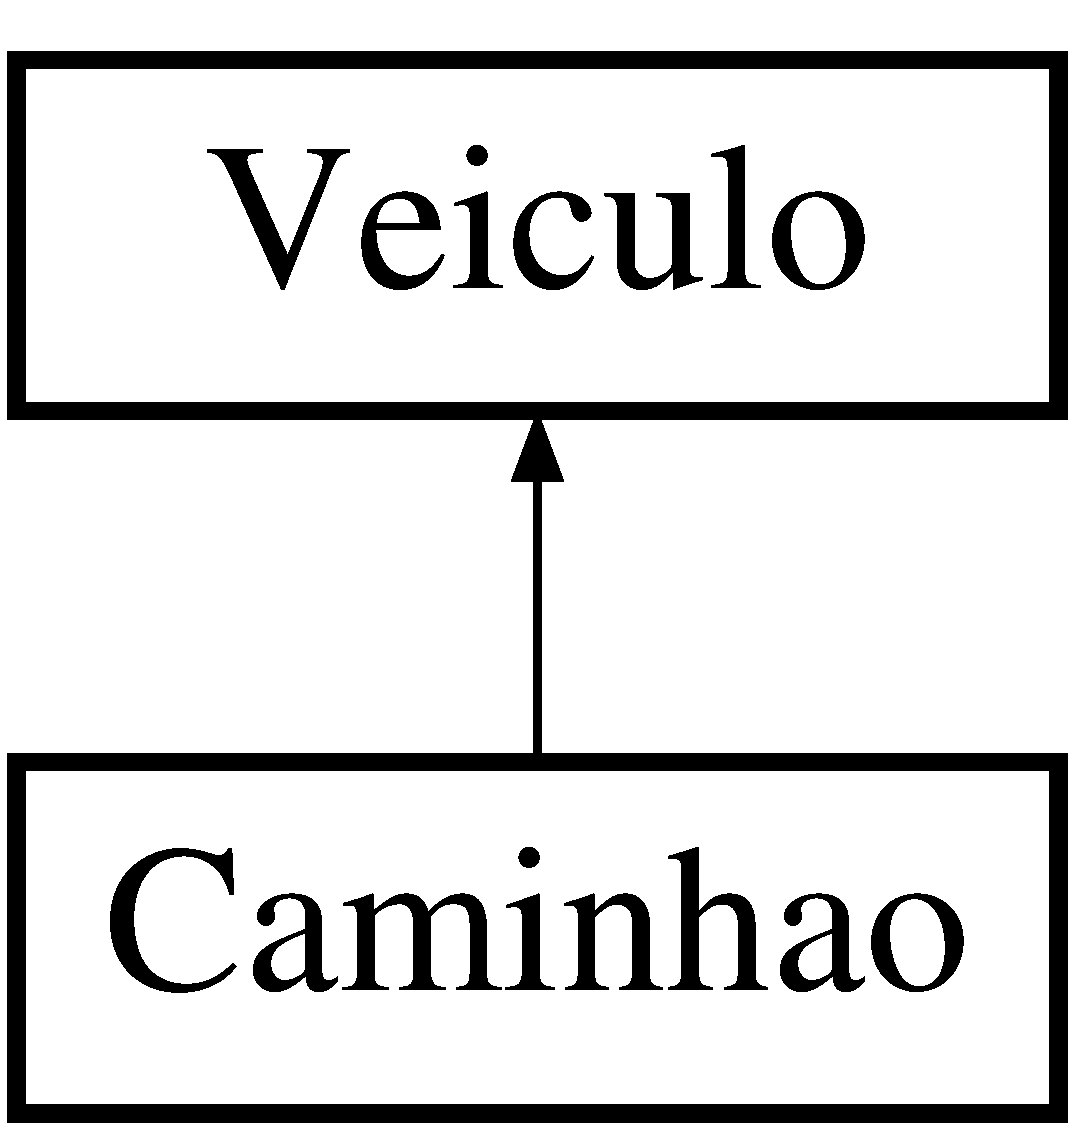
\includegraphics[height=2.000000cm]{class_caminhao}
\end{center}
\end{figure}
\subsection*{Membros públicos}
\begin{DoxyCompactItemize}
\item 
\mbox{\hyperlink{class_caminhao_af533c39b3db0b14e7c404d4d91a88e47}{Caminhao}} ()
\begin{DoxyCompactList}\small\item\em construtor padrão com capacidade de carga aleatória \end{DoxyCompactList}\end{DoxyCompactItemize}
\subsection*{Atributos Protegidos}
\begin{DoxyCompactItemize}
\item 
\mbox{\Hypertarget{class_caminhao_a32551c3ccafebc3d06ecb130e6c7cbb5}\label{class_caminhao_a32551c3ccafebc3d06ecb130e6c7cbb5}} 
int {\bfseries capacidade\+Carga}
\end{DoxyCompactItemize}


\subsection{Documentação dos Construtores \& Destrutor}
\mbox{\Hypertarget{class_caminhao_af533c39b3db0b14e7c404d4d91a88e47}\label{class_caminhao_af533c39b3db0b14e7c404d4d91a88e47}} 
\index{Caminhao@{Caminhao}!Caminhao@{Caminhao}}
\index{Caminhao@{Caminhao}!Caminhao@{Caminhao}}
\subsubsection{\texorpdfstring{Caminhao()}{Caminhao()}}
{\footnotesize\ttfamily Caminhao.\+Caminhao (\begin{DoxyParamCaption}{ }\end{DoxyParamCaption})}



construtor padrão com capacidade de carga aleatória 

chama construtor padrão da classe pai 

A documentação para esta classe foi gerada a partir do seguinte ficheiro\+:\begin{DoxyCompactItemize}
\item 
/\+Users/evertoncardoso/\+Desktop/\+Doc/Caminhao.\+java\end{DoxyCompactItemize}

\hypertarget{class_carro}{}\section{Referência à classe Carro}
\label{class_carro}\index{Carro@{Carro}}
Diagrama de heranças da classe Carro\begin{figure}[H]
\begin{center}
\leavevmode
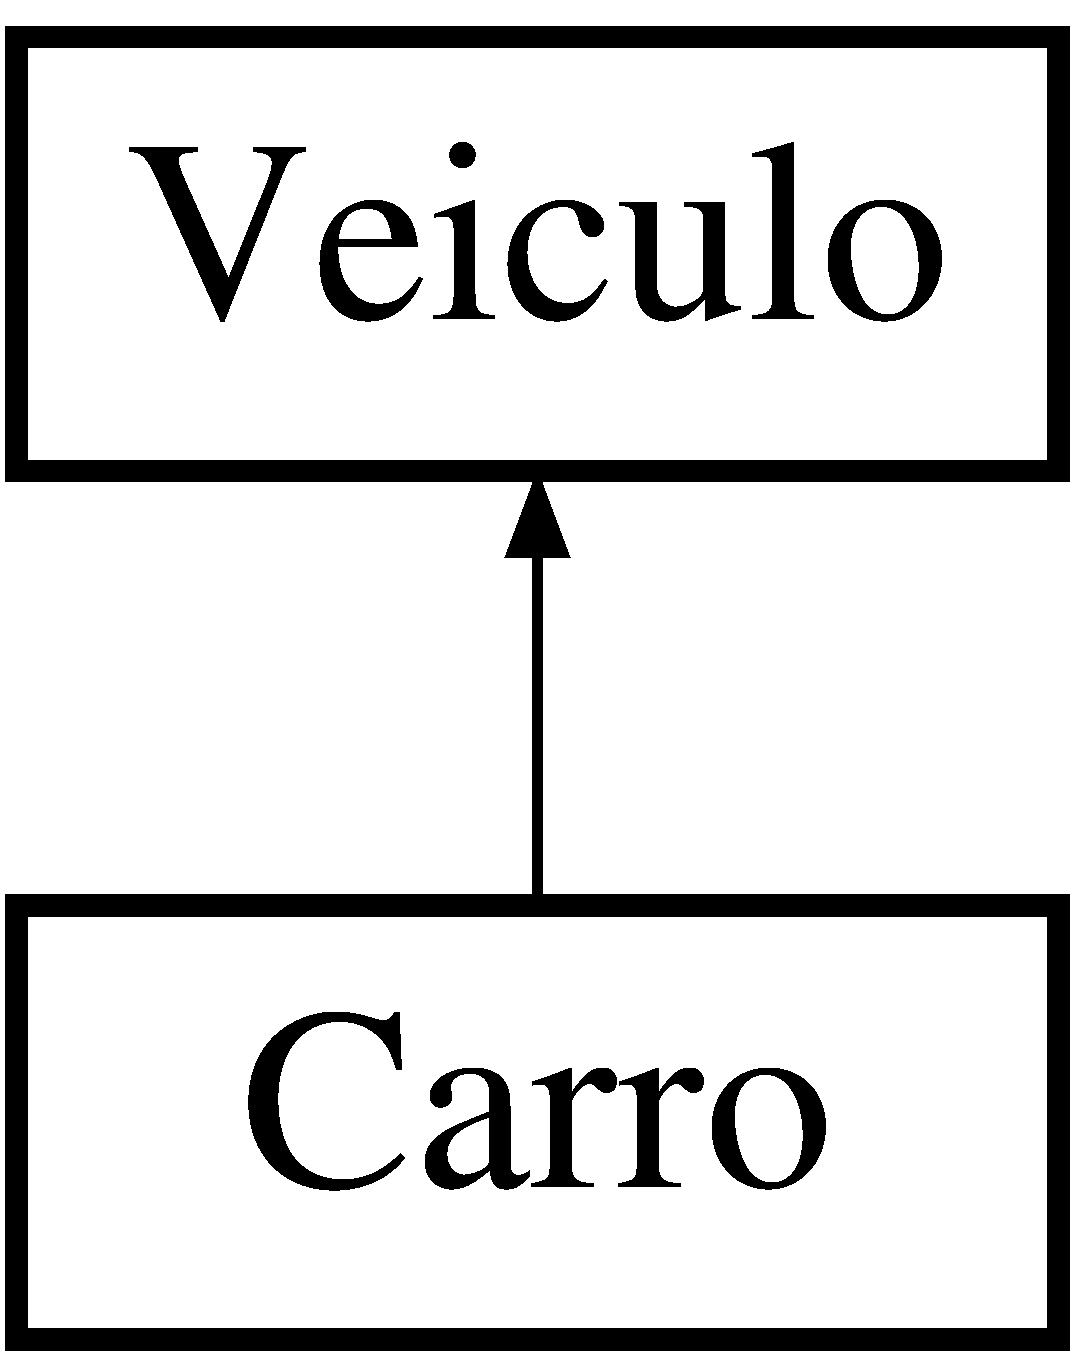
\includegraphics[height=2.000000cm]{class_carro}
\end{center}
\end{figure}
\subsection*{Membros públicos}
\begin{DoxyCompactItemize}
\item 
\mbox{\hyperlink{class_carro_a853f79365b5c36491d34cf8f3815f75e}{Carro}} ()
\begin{DoxyCompactList}\small\item\em construtor padrão com número de passageiros aleatório \end{DoxyCompactList}\end{DoxyCompactItemize}
\subsection*{Atributos Protegidos}
\begin{DoxyCompactItemize}
\item 
\mbox{\Hypertarget{class_carro_a078d618deb133f1bd65f421c10c77507}\label{class_carro_a078d618deb133f1bd65f421c10c77507}} 
int {\bfseries num\+Passageiros}
\end{DoxyCompactItemize}


\subsection{Documentação dos Construtores \& Destrutor}
\mbox{\Hypertarget{class_carro_a853f79365b5c36491d34cf8f3815f75e}\label{class_carro_a853f79365b5c36491d34cf8f3815f75e}} 
\index{Carro@{Carro}!Carro@{Carro}}
\index{Carro@{Carro}!Carro@{Carro}}
\subsubsection{\texorpdfstring{Carro()}{Carro()}}
{\footnotesize\ttfamily Carro.\+Carro (\begin{DoxyParamCaption}{ }\end{DoxyParamCaption})}



construtor padrão com número de passageiros aleatório 

passa dados para o construtor padrão de veiculos 

A documentação para esta classe foi gerada a partir do seguinte ficheiro\+:\begin{DoxyCompactItemize}
\item 
/\+Users/evertoncardoso/\+Desktop/\+Doc/Carro.\+java\end{DoxyCompactItemize}

\hypertarget{class_colisoes}{}\section{Referência à classe Colisoes}
\label{class_colisoes}\index{Colisoes@{Colisoes}}
\subsection*{Membros públicos}
\begin{DoxyCompactItemize}
\item 
\mbox{\hyperlink{class_colisoes_a8a51b610e7e5d3a011b5c790429dc598}{Colisoes}} ()
\begin{DoxyCompactList}\small\item\em construtor padrão \end{DoxyCompactList}\item 
\mbox{\Hypertarget{class_colisoes_a12b4feebe3aceaf64b6a20941677d31f}\label{class_colisoes_a12b4feebe3aceaf64b6a20941677d31f}} 
String \mbox{\hyperlink{class_colisoes_a12b4feebe3aceaf64b6a20941677d31f}{get\+Tipo}} (int i, int j)
\begin{DoxyCompactList}\small\item\em retorna o tipo que está nas coordenadas entradas \end{DoxyCompactList}\item 
\mbox{\Hypertarget{class_colisoes_a2a5dc91b1a181819919be8726272293a}\label{class_colisoes_a2a5dc91b1a181819919be8726272293a}} 
int \mbox{\hyperlink{class_colisoes_a2a5dc91b1a181819919be8726272293a}{get\+ID}} (int i, int j)
\begin{DoxyCompactList}\small\item\em retorna a ID que está nas coordenadas entradas \end{DoxyCompactList}\item 
\mbox{\Hypertarget{class_colisoes_aee76e39346a03b3f6eeddbca2efe8067}\label{class_colisoes_aee76e39346a03b3f6eeddbca2efe8067}} 
void \mbox{\hyperlink{class_colisoes_aee76e39346a03b3f6eeddbca2efe8067}{ocupado}} (int i, int j, String tipo, int ID)
\begin{DoxyCompactList}\small\item\em popula a coordenada entrada com o tipo e ID desejado \end{DoxyCompactList}\item 
\mbox{\Hypertarget{class_colisoes_ad901b8e1997c5166cf91e1571fc8a9b9}\label{class_colisoes_ad901b8e1997c5166cf91e1571fc8a9b9}} 
void {\bfseries restaura} (int i, int j)
\end{DoxyCompactItemize}
\subsection*{Atributos Protegidos}
\begin{DoxyCompactItemize}
\item 
\mbox{\Hypertarget{class_colisoes_a44a61dfac2eac26a202bc861c07b3b04}\label{class_colisoes_a44a61dfac2eac26a202bc861c07b3b04}} 
String {\bfseries tipos} \mbox{[}$\,$\mbox{]}\mbox{[}$\,$\mbox{]}
\item 
\mbox{\Hypertarget{class_colisoes_a24e82ed4cd735cdf7adc0e1dfe1da0d4}\label{class_colisoes_a24e82ed4cd735cdf7adc0e1dfe1da0d4}} 
int {\bfseries id} \mbox{[}$\,$\mbox{]}\mbox{[}$\,$\mbox{]}
\end{DoxyCompactItemize}


\subsection{Documentação dos Construtores \& Destrutor}
\mbox{\Hypertarget{class_colisoes_a8a51b610e7e5d3a011b5c790429dc598}\label{class_colisoes_a8a51b610e7e5d3a011b5c790429dc598}} 
\index{Colisoes@{Colisoes}!Colisoes@{Colisoes}}
\index{Colisoes@{Colisoes}!Colisoes@{Colisoes}}
\subsubsection{\texorpdfstring{Colisoes()}{Colisoes()}}
{\footnotesize\ttfamily Colisoes.\+Colisoes (\begin{DoxyParamCaption}{ }\end{DoxyParamCaption})}



construtor padrão 

nova matriz de 30x60 para armazenar os tipos de veiculos

nova matriz de 30x60 para armazenar as I\+Ds dos veiculos

inicializa as duas matrizes como vazias 

A documentação para esta classe foi gerada a partir do seguinte ficheiro\+:\begin{DoxyCompactItemize}
\item 
/\+Users/evertoncardoso/\+Desktop/\+Doc/Colisoes.\+java\end{DoxyCompactItemize}

\hypertarget{class_legenda}{}\section{Referência à classe Legenda}
\label{class_legenda}\index{Legenda@{Legenda}}
\subsection*{Membros públicos}
\begin{DoxyCompactItemize}
\item 
void \mbox{\hyperlink{class_legenda_a213202792f82e028c9e144aadad36ee9}{exibe\+Legenda}} ()
\begin{DoxyCompactList}\small\item\em Exibe o mundo sem nenhum veiculo, indicando as fabricas (é exibido por 5 segundos) \end{DoxyCompactList}\item 
void \mbox{\hyperlink{class_legenda_ad2b8f204bbb24bf96a198f5e76e908fe}{volta\+Carro}} ()
\begin{DoxyCompactList}\small\item\em volta o carro do terminal uma linha acima \end{DoxyCompactList}\item 
void \mbox{\hyperlink{class_legenda_a30586aa3859ac3880a8f5d2acc7a5cb5}{pausa\+Legenda}} ()
\begin{DoxyCompactList}\small\item\em pausa a execução do programa por 5 segundos \end{DoxyCompactList}\item 
void \mbox{\hyperlink{class_legenda_a0c879e1772bd84a55e9c1cca7d5678dc}{volta\+Comeco\+Legenda}} ()
\begin{DoxyCompactList}\small\item\em volta o carro para o inicio do mapa \end{DoxyCompactList}\end{DoxyCompactItemize}


\subsection{Documentação dos métodos}
\mbox{\Hypertarget{class_legenda_a213202792f82e028c9e144aadad36ee9}\label{class_legenda_a213202792f82e028c9e144aadad36ee9}} 
\index{Legenda@{Legenda}!exibe\+Legenda@{exibe\+Legenda}}
\index{exibe\+Legenda@{exibe\+Legenda}!Legenda@{Legenda}}
\subsubsection{\texorpdfstring{exibe\+Legenda()}{exibeLegenda()}}
{\footnotesize\ttfamily void Legenda.\+exibe\+Legenda (\begin{DoxyParamCaption}{ }\end{DoxyParamCaption})}



Exibe o mundo sem nenhum veiculo, indicando as fabricas (é exibido por 5 segundos) 

Grafo de chamadas desta função\+:
% FIG 0
Este é o diagrama das funções que utilizam esta função\+:
% FIG 1
\mbox{\Hypertarget{class_legenda_a30586aa3859ac3880a8f5d2acc7a5cb5}\label{class_legenda_a30586aa3859ac3880a8f5d2acc7a5cb5}} 
\index{Legenda@{Legenda}!pausa\+Legenda@{pausa\+Legenda}}
\index{pausa\+Legenda@{pausa\+Legenda}!Legenda@{Legenda}}
\subsubsection{\texorpdfstring{pausa\+Legenda()}{pausaLegenda()}}
{\footnotesize\ttfamily void Legenda.\+pausa\+Legenda (\begin{DoxyParamCaption}{ }\end{DoxyParamCaption})}



pausa a execução do programa por 5 segundos 

Este é o diagrama das funções que utilizam esta função\+:
% FIG 2
\mbox{\Hypertarget{class_legenda_ad2b8f204bbb24bf96a198f5e76e908fe}\label{class_legenda_ad2b8f204bbb24bf96a198f5e76e908fe}} 
\index{Legenda@{Legenda}!volta\+Carro@{volta\+Carro}}
\index{volta\+Carro@{volta\+Carro}!Legenda@{Legenda}}
\subsubsection{\texorpdfstring{volta\+Carro()}{voltaCarro()}}
{\footnotesize\ttfamily void Legenda.\+volta\+Carro (\begin{DoxyParamCaption}{ }\end{DoxyParamCaption})}



volta o carro do terminal uma linha acima 

Este é o diagrama das funções que utilizam esta função\+:
% FIG 3
\mbox{\Hypertarget{class_legenda_a0c879e1772bd84a55e9c1cca7d5678dc}\label{class_legenda_a0c879e1772bd84a55e9c1cca7d5678dc}} 
\index{Legenda@{Legenda}!volta\+Comeco\+Legenda@{volta\+Comeco\+Legenda}}
\index{volta\+Comeco\+Legenda@{volta\+Comeco\+Legenda}!Legenda@{Legenda}}
\subsubsection{\texorpdfstring{volta\+Comeco\+Legenda()}{voltaComecoLegenda()}}
{\footnotesize\ttfamily void Legenda.\+volta\+Comeco\+Legenda (\begin{DoxyParamCaption}{ }\end{DoxyParamCaption})}



volta o carro para o inicio do mapa 

Este é o diagrama das funções que utilizam esta função\+:
% FIG 4


A documentação para esta classe foi gerada a partir do seguinte ficheiro\+:\begin{DoxyCompactItemize}
\item 
/\+Users/evertoncardoso/\+Desktop/\+Doc/\mbox{\hyperlink{_legenda_8java}{Legenda.\+java}}\end{DoxyCompactItemize}

\hypertarget{class_main}{}\section{Referência à classe Main}
\label{class_main}\index{Main@{Main}}
\subsection*{Membros públicos estáticos}
\begin{DoxyCompactItemize}
\item 
static void \mbox{\hyperlink{class_main_a54c9709d2de6897d6f13e9af08ef177f}{main}} (String argv\mbox{[}$\,$\mbox{]})
\end{DoxyCompactItemize}


\subsection{Documentação dos métodos}
\mbox{\Hypertarget{class_main_a54c9709d2de6897d6f13e9af08ef177f}\label{class_main_a54c9709d2de6897d6f13e9af08ef177f}} 
\index{Main@{Main}!main@{main}}
\index{main@{main}!Main@{Main}}
\subsubsection{\texorpdfstring{main()}{main()}}
{\footnotesize\ttfamily static void Main.\+main (\begin{DoxyParamCaption}\item[{String}]{argv\mbox{[}$\,$\mbox{]} }\end{DoxyParamCaption})\hspace{0.3cm}{\ttfamily [static]}}

cria o objeto mundo

novo vetor dinâmico para armazenar os carros

novo vetor dinâmico para armazenar os caminhões

novo vetor dinâmico para armazenar as motos

vetor que salva a quantidade de objetos apagados. Indice 0 = caminhões, indice 1 = carros, indice 2 = motos

vetor que salva a quantidade de objetos criados. Indice 0 = caminhões, indice 1 = carros, indice 2 = motos

cria 10 carros, caminhões e motos

loop infinito de execução do programa

cria um novo objeto detector de colisões

cria um novo vetor dinâmico para armazenar as I\+Ds a serem apagadas

imprime a quantidade de caminhões, carros e motos no mundo atualmente

detecta colisões entre caminhões e outros veiculos e armazena os I\+DS dos objetos a serem apagados.

detecta colisões entre carros e outros veiculos e armazena os I\+DS dos objetos a serem apagados.

detecta colisões entre motos e outros veiculos e armazena os I\+DS dos objetos a serem apagados.

apaga todos os objetos com as I\+Ds salvas na lista de colisões e incrementa no vetor de apagados total.

popula o mundo de caminhões, conta quantos novos devem ser criados e move os existentes

cria os novos caminhões e incrementa o vetor de criados total

popula o mundo de carros, conta quantos novos devem ser criados e move os existentes

cria os novos carros e incrementa o vetor de criados total

popula o mundo de motos, conta quantos novos devem ser criados e move os existentes

cria as novas motos e incrementa o vetor de criados total

desenha o mundo no console

exibe quantos veiculos foram apagados e criados durante a execução do programa

pausa o console pelo tempo determinado

volta o cursor para o começo do console

reinicia a matriz do mundo. 

A documentação para esta classe foi gerada a partir do seguinte ficheiro\+:\begin{DoxyCompactItemize}
\item 
/\+Users/evertoncardoso/\+Desktop/\+Doc/Main.\+java\end{DoxyCompactItemize}

\hypertarget{class_moto}{}\section{Referência à classe Moto}
\label{class_moto}\index{Moto@{Moto}}
Diagrama de heranças da classe Moto\begin{figure}[H]
\begin{center}
\leavevmode
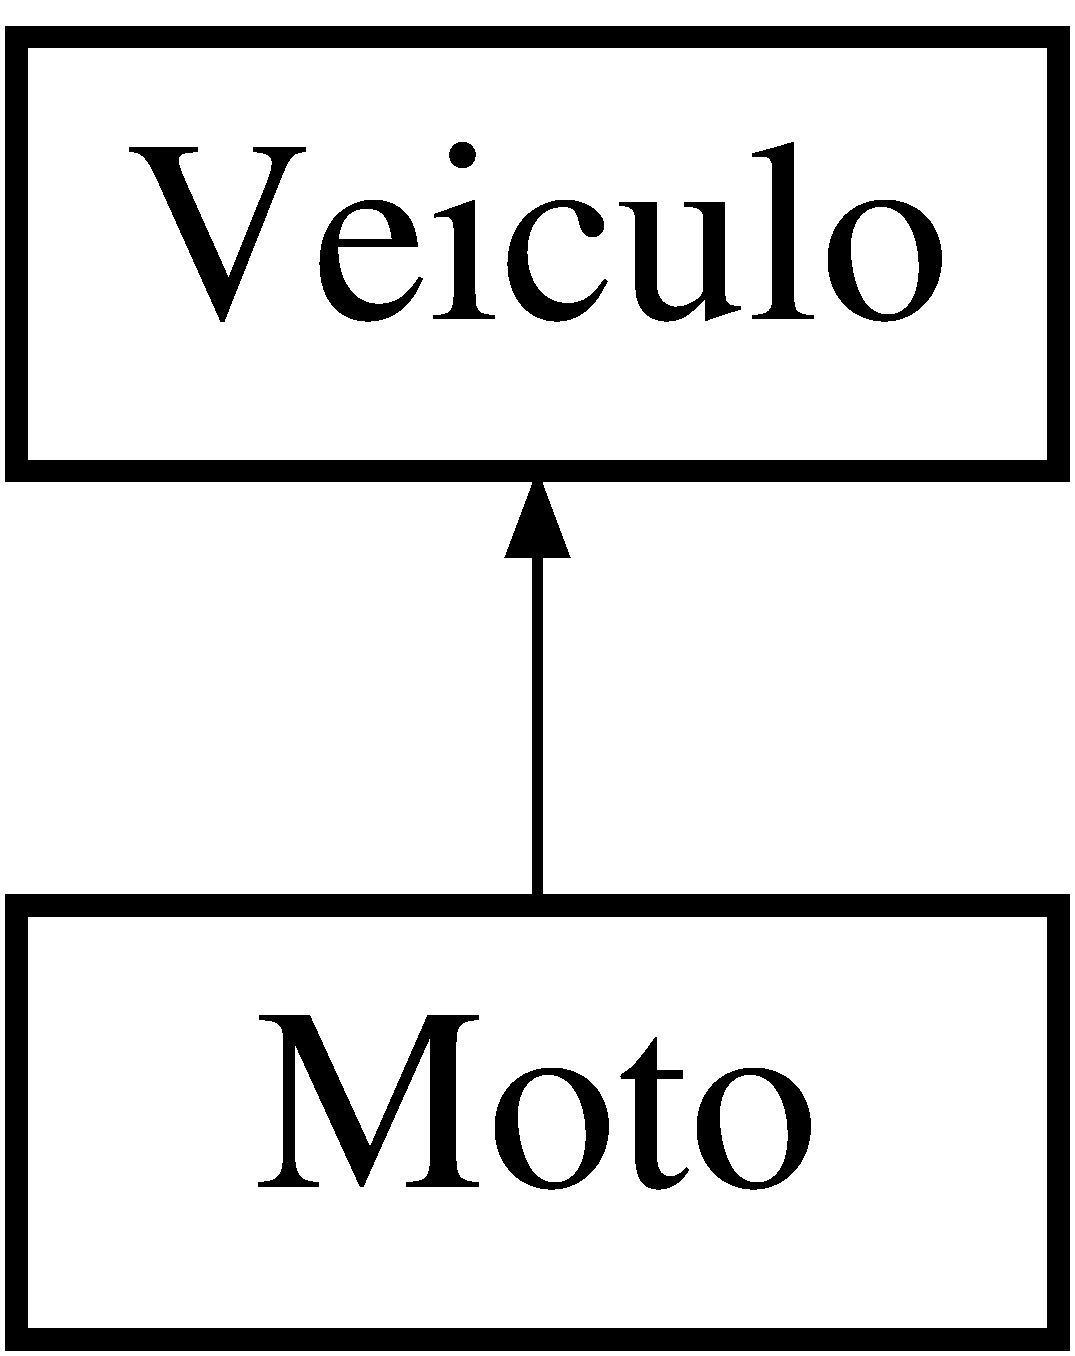
\includegraphics[height=2.000000cm]{class_moto}
\end{center}
\end{figure}
\subsection*{Membros públicos}
\begin{DoxyCompactItemize}
\item 
\mbox{\hyperlink{class_moto_af900d6c1d6b9a69fb6b8bdb0c3401603}{Moto}} ()
\begin{DoxyCompactList}\small\item\em construtor padrão com tipo da moto aleatória \end{DoxyCompactList}\end{DoxyCompactItemize}
\subsection*{Atributos Protegidos}
\begin{DoxyCompactItemize}
\item 
\mbox{\Hypertarget{class_moto_a98533b801c6277bdac415e9d21f74efe}\label{class_moto_a98533b801c6277bdac415e9d21f74efe}} 
String {\bfseries tipo}
\end{DoxyCompactItemize}


\subsection{Documentação dos Construtores \& Destrutor}
\mbox{\Hypertarget{class_moto_af900d6c1d6b9a69fb6b8bdb0c3401603}\label{class_moto_af900d6c1d6b9a69fb6b8bdb0c3401603}} 
\index{Moto@{Moto}!Moto@{Moto}}
\index{Moto@{Moto}!Moto@{Moto}}
\subsubsection{\texorpdfstring{Moto()}{Moto()}}
{\footnotesize\ttfamily Moto.\+Moto (\begin{DoxyParamCaption}{ }\end{DoxyParamCaption})}



construtor padrão com tipo da moto aleatória 

chama construtor padrão da classe pai 

A documentação para esta classe foi gerada a partir do seguinte ficheiro\+:\begin{DoxyCompactItemize}
\item 
/\+Users/evertoncardoso/\+Desktop/\+Doc/Moto.\+java\end{DoxyCompactItemize}

\hypertarget{class_mundo}{}\section{Referência à classe Mundo}
\label{class_mundo}\index{Mundo@{Mundo}}
\subsection*{Membros públicos}
\begin{DoxyCompactItemize}
\item 
\mbox{\hyperlink{class_mundo_ae3801a0a633ad3475456c67639561105}{Mundo}} ()
\begin{DoxyCompactList}\small\item\em construtor padrão \end{DoxyCompactList}\item 
void \mbox{\hyperlink{class_mundo_a6e10fa6c3ae633a67e2ba897d83ab951}{reinicia\+Mundo}} ()
\begin{DoxyCompactList}\small\item\em reinicia a matriz mundo para a matriz padrão \end{DoxyCompactList}\item 
void \mbox{\hyperlink{class_mundo_adbafcb32f5f209eda97e1c7953c6e599}{desenha\+Mundo}} ()
\begin{DoxyCompactList}\small\item\em imprime no console a matriz com as cores e posições pré definidas \end{DoxyCompactList}\item 
void \mbox{\hyperlink{class_mundo_afec47a52ae6772f201f120fc62ba4546}{insere\+No\+Mundo}} (int x, int y, int tipo)
\begin{DoxyCompactList}\small\item\em insere um veiculo na matriz do mundo na posição indicada \end{DoxyCompactList}\item 
void \mbox{\hyperlink{class_mundo_a546c0413297120b08815afafcc0e7d32}{volta\+Comeco}} ()
\begin{DoxyCompactList}\small\item\em volta o cursor no console para o começo \end{DoxyCompactList}\item 
int \mbox{\hyperlink{class_mundo_ac971ab63c34c7ab0c00df63277589338}{get\+Localizacao}} (int x, int y)
\begin{DoxyCompactList}\small\item\em retorna que tipo esta salvo nas coordenadas indicadas \end{DoxyCompactList}\item 
void \mbox{\hyperlink{class_mundo_a871bfb3ebd38d8ce498777bb0dd1cdeb}{pausa\+Mundo}} ()
\begin{DoxyCompactList}\small\item\em pausa a execução do programa por 0,5s \end{DoxyCompactList}\end{DoxyCompactItemize}
\subsection*{Atributos Protegidos}
\begin{DoxyCompactItemize}
\item 
int \mbox{\hyperlink{class_mundo_a689dcc4a20afc97fc8a63907ab682d7e}{mundo}} \mbox{[}$\,$\mbox{]}\mbox{[}$\,$\mbox{]}
\end{DoxyCompactItemize}


\subsection{Documentação dos Construtores \& Destrutor}
\mbox{\Hypertarget{class_mundo_ae3801a0a633ad3475456c67639561105}\label{class_mundo_ae3801a0a633ad3475456c67639561105}} 
\index{Mundo@{Mundo}!Mundo@{Mundo}}
\index{Mundo@{Mundo}!Mundo@{Mundo}}
\subsubsection{\texorpdfstring{Mundo()}{Mundo()}}
{\footnotesize\ttfamily Mundo.\+Mundo (\begin{DoxyParamCaption}{ }\end{DoxyParamCaption})}



construtor padrão 

cria a matriz mundo padrão Grafo de chamadas desta função\+:
% FIG 0


\subsection{Documentação dos métodos}
\mbox{\Hypertarget{class_mundo_adbafcb32f5f209eda97e1c7953c6e599}\label{class_mundo_adbafcb32f5f209eda97e1c7953c6e599}} 
\index{Mundo@{Mundo}!desenha\+Mundo@{desenha\+Mundo}}
\index{desenha\+Mundo@{desenha\+Mundo}!Mundo@{Mundo}}
\subsubsection{\texorpdfstring{desenha\+Mundo()}{desenhaMundo()}}
{\footnotesize\ttfamily void Mundo.\+desenha\+Mundo (\begin{DoxyParamCaption}{ }\end{DoxyParamCaption})}



imprime no console a matriz com as cores e posições pré definidas 

bordas vermelhas

fundo preto

fabrica verde

moto marrom

carro azul

caminhao cinza Este é o diagrama das funções que utilizam esta função\+:
% FIG 1
\mbox{\Hypertarget{class_mundo_ac971ab63c34c7ab0c00df63277589338}\label{class_mundo_ac971ab63c34c7ab0c00df63277589338}} 
\index{Mundo@{Mundo}!get\+Localizacao@{get\+Localizacao}}
\index{get\+Localizacao@{get\+Localizacao}!Mundo@{Mundo}}
\subsubsection{\texorpdfstring{get\+Localizacao()}{getLocalizacao()}}
{\footnotesize\ttfamily int Mundo.\+get\+Localizacao (\begin{DoxyParamCaption}\item[{int}]{x,  }\item[{int}]{y }\end{DoxyParamCaption})}



retorna que tipo esta salvo nas coordenadas indicadas 

Este é o diagrama das funções que utilizam esta função\+:
% FIG 2
\mbox{\Hypertarget{class_mundo_afec47a52ae6772f201f120fc62ba4546}\label{class_mundo_afec47a52ae6772f201f120fc62ba4546}} 
\index{Mundo@{Mundo}!insere\+No\+Mundo@{insere\+No\+Mundo}}
\index{insere\+No\+Mundo@{insere\+No\+Mundo}!Mundo@{Mundo}}
\subsubsection{\texorpdfstring{insere\+No\+Mundo()}{insereNoMundo()}}
{\footnotesize\ttfamily void Mundo.\+insere\+No\+Mundo (\begin{DoxyParamCaption}\item[{int}]{x,  }\item[{int}]{y,  }\item[{int}]{tipo }\end{DoxyParamCaption})}



insere um veiculo na matriz do mundo na posição indicada 

Este é o diagrama das funções que utilizam esta função\+:
% FIG 3
\mbox{\Hypertarget{class_mundo_a871bfb3ebd38d8ce498777bb0dd1cdeb}\label{class_mundo_a871bfb3ebd38d8ce498777bb0dd1cdeb}} 
\index{Mundo@{Mundo}!pausa\+Mundo@{pausa\+Mundo}}
\index{pausa\+Mundo@{pausa\+Mundo}!Mundo@{Mundo}}
\subsubsection{\texorpdfstring{pausa\+Mundo()}{pausaMundo()}}
{\footnotesize\ttfamily void Mundo.\+pausa\+Mundo (\begin{DoxyParamCaption}{ }\end{DoxyParamCaption})}



pausa a execução do programa por 0,5s 

Este é o diagrama das funções que utilizam esta função\+:
% FIG 4
\mbox{\Hypertarget{class_mundo_a6e10fa6c3ae633a67e2ba897d83ab951}\label{class_mundo_a6e10fa6c3ae633a67e2ba897d83ab951}} 
\index{Mundo@{Mundo}!reinicia\+Mundo@{reinicia\+Mundo}}
\index{reinicia\+Mundo@{reinicia\+Mundo}!Mundo@{Mundo}}
\subsubsection{\texorpdfstring{reinicia\+Mundo()}{reiniciaMundo()}}
{\footnotesize\ttfamily void Mundo.\+reinicia\+Mundo (\begin{DoxyParamCaption}{ }\end{DoxyParamCaption})}



reinicia a matriz mundo para a matriz padrão 

Este é o diagrama das funções que utilizam esta função\+:
% FIG 5
\mbox{\Hypertarget{class_mundo_a546c0413297120b08815afafcc0e7d32}\label{class_mundo_a546c0413297120b08815afafcc0e7d32}} 
\index{Mundo@{Mundo}!volta\+Comeco@{volta\+Comeco}}
\index{volta\+Comeco@{volta\+Comeco}!Mundo@{Mundo}}
\subsubsection{\texorpdfstring{volta\+Comeco()}{voltaComeco()}}
{\footnotesize\ttfamily void Mundo.\+volta\+Comeco (\begin{DoxyParamCaption}{ }\end{DoxyParamCaption})}



volta o cursor no console para o começo 

Este é o diagrama das funções que utilizam esta função\+:
% FIG 6


\subsection{Documentação dos dados membro}
\mbox{\Hypertarget{class_mundo_a689dcc4a20afc97fc8a63907ab682d7e}\label{class_mundo_a689dcc4a20afc97fc8a63907ab682d7e}} 
\index{Mundo@{Mundo}!mundo@{mundo}}
\index{mundo@{mundo}!Mundo@{Mundo}}
\subsubsection{\texorpdfstring{mundo}{mundo}}
{\footnotesize\ttfamily int Mundo.\+mundo\mbox{[}$\,$\mbox{]}\mbox{[}$\,$\mbox{]}\hspace{0.3cm}{\ttfamily [protected]}}



A documentação para esta classe foi gerada a partir do seguinte ficheiro\+:\begin{DoxyCompactItemize}
\item 
/\+Users/evertoncardoso/\+Desktop/\+Doc/\mbox{\hyperlink{_mundo_8java}{Mundo.\+java}}\end{DoxyCompactItemize}

\hypertarget{class_veiculo}{}\section{Referência à classe Veiculo}
\label{class_veiculo}\index{Veiculo@{Veiculo}}
Diagrama de heranças da classe Veiculo\begin{figure}[H]
\begin{center}
\leavevmode
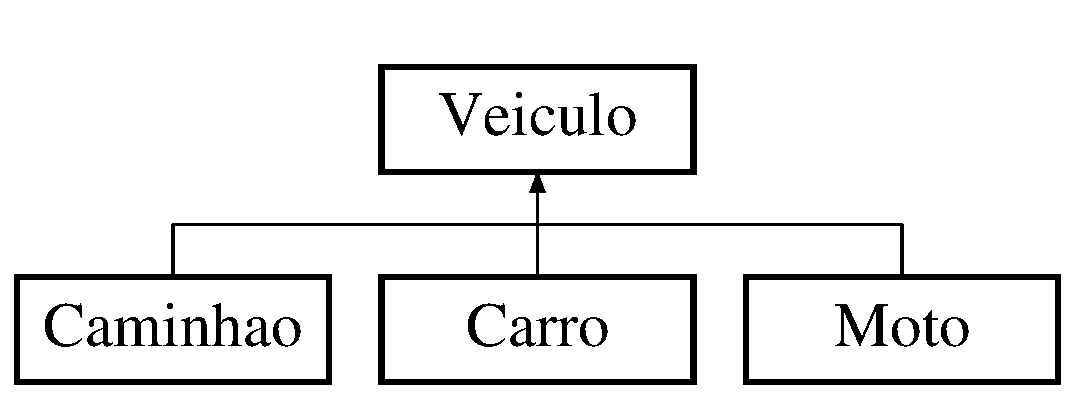
\includegraphics[height=2.000000cm]{class_veiculo}
\end{center}
\end{figure}
\subsection*{Membros públicos}
\begin{DoxyCompactItemize}
\item 
\mbox{\hyperlink{class_veiculo_a6e43a5035741a90e4ef9d07b7fce6c87}{Veiculo}} (int velocidade, String cor)
\begin{DoxyCompactList}\small\item\em construtor padrão \end{DoxyCompactList}\item 
\mbox{\Hypertarget{class_veiculo_a2bb3cf76255e4d6c33531daa82b1dfa7}\label{class_veiculo_a2bb3cf76255e4d6c33531daa82b1dfa7}} 
void \mbox{\hyperlink{class_veiculo_a2bb3cf76255e4d6c33531daa82b1dfa7}{dentro\+Da\+Fabrica}} ()
\begin{DoxyCompactList}\small\item\em define o objeto como dentro da fabrica \end{DoxyCompactList}\item 
\mbox{\Hypertarget{class_veiculo_a72e8117111488e80a40e377327c361ea}\label{class_veiculo_a72e8117111488e80a40e377327c361ea}} 
void \mbox{\hyperlink{class_veiculo_a72e8117111488e80a40e377327c361ea}{fora\+Da\+Fabrica}} ()
\begin{DoxyCompactList}\small\item\em define o objeto como fora da fabrica \end{DoxyCompactList}\item 
void \mbox{\hyperlink{class_veiculo_a3341b0ed6b4d34db990a31f7a499ae80}{move}} ()
\begin{DoxyCompactList}\small\item\em move o objeto para uma direção aleatória (direita, esquerda, cima ou baixo), respeitando sua velocidade \end{DoxyCompactList}\item 
\mbox{\Hypertarget{class_veiculo_a235b29e1e25ec8c769b20fb2aeba8404}\label{class_veiculo_a235b29e1e25ec8c769b20fb2aeba8404}} 
int \mbox{\hyperlink{class_veiculo_a235b29e1e25ec8c769b20fb2aeba8404}{getX}} ()
\begin{DoxyCompactList}\small\item\em volta a posição X \end{DoxyCompactList}\item 
\mbox{\Hypertarget{class_veiculo_a06b2a923e51186673a016f75d10363d3}\label{class_veiculo_a06b2a923e51186673a016f75d10363d3}} 
int \mbox{\hyperlink{class_veiculo_a06b2a923e51186673a016f75d10363d3}{getY}} ()
\begin{DoxyCompactList}\small\item\em volta a posição Y \end{DoxyCompactList}\item 
\mbox{\Hypertarget{class_veiculo_a6447f0eeb99399f1f96e835c22a88479}\label{class_veiculo_a6447f0eeb99399f1f96e835c22a88479}} 
boolean \mbox{\hyperlink{class_veiculo_a6447f0eeb99399f1f96e835c22a88479}{get\+Fabrica}} ()
\begin{DoxyCompactList}\small\item\em volta o boleano fabrica (true para dentro e false para fora) \end{DoxyCompactList}\item 
\mbox{\Hypertarget{class_veiculo_a09c389362736b3ca90a0200e01545e73}\label{class_veiculo_a09c389362736b3ca90a0200e01545e73}} 
int \mbox{\hyperlink{class_veiculo_a09c389362736b3ca90a0200e01545e73}{get\+Id}} ()
\begin{DoxyCompactList}\small\item\em volta a ID do objeto \end{DoxyCompactList}\end{DoxyCompactItemize}
\subsection*{Atributos Protegidos}
\begin{DoxyCompactItemize}
\item 
\mbox{\Hypertarget{class_veiculo_a069917a284297fe5b385258b2afd9ad6}\label{class_veiculo_a069917a284297fe5b385258b2afd9ad6}} 
int {\bfseries x}
\item 
\mbox{\Hypertarget{class_veiculo_a23d377a69bdf558ebedb5bc35dcdebf5}\label{class_veiculo_a23d377a69bdf558ebedb5bc35dcdebf5}} 
boolean {\bfseries fabrica}
\item 
\mbox{\Hypertarget{class_veiculo_a6bc5886e61340672e69bd638936ec1d5}\label{class_veiculo_a6bc5886e61340672e69bd638936ec1d5}} 
String {\bfseries cor}
\end{DoxyCompactItemize}


\subsection{Documentação dos Construtores \& Destrutor}
\mbox{\Hypertarget{class_veiculo_a6e43a5035741a90e4ef9d07b7fce6c87}\label{class_veiculo_a6e43a5035741a90e4ef9d07b7fce6c87}} 
\index{Veiculo@{Veiculo}!Veiculo@{Veiculo}}
\index{Veiculo@{Veiculo}!Veiculo@{Veiculo}}
\subsubsection{\texorpdfstring{Veiculo()}{Veiculo()}}
{\footnotesize\ttfamily Veiculo.\+Veiculo (\begin{DoxyParamCaption}\item[{int}]{velocidade,  }\item[{String}]{cor }\end{DoxyParamCaption})}



construtor padrão 

define a cor

define a velocidade

cria um objeto aleatorio

randomiza a posição X

randomiza a posição Y

define o objeto como fora da fabrica

cria um ID aleatório 

\subsection{Documentação dos métodos}
\mbox{\Hypertarget{class_veiculo_a3341b0ed6b4d34db990a31f7a499ae80}\label{class_veiculo_a3341b0ed6b4d34db990a31f7a499ae80}} 
\index{Veiculo@{Veiculo}!move@{move}}
\index{move@{move}!Veiculo@{Veiculo}}
\subsubsection{\texorpdfstring{move()}{move()}}
{\footnotesize\ttfamily void Veiculo.\+move (\begin{DoxyParamCaption}{ }\end{DoxyParamCaption})}



move o objeto para uma direção aleatória (direita, esquerda, cima ou baixo), respeitando sua velocidade 

move para a direita

move para a esquerda

move para baixo

move para cima 

A documentação para esta classe foi gerada a partir do seguinte ficheiro\+:\begin{DoxyCompactItemize}
\item 
/\+Users/evertoncardoso/\+Desktop/\+Doc/Veiculo.\+java\end{DoxyCompactItemize}

\chapter{Documentação do ficheiro}
\hypertarget{_aleatorio_8java}{}\section{Referência ao ficheiro /\+Users/evertoncardoso/\+Desktop/\+Doc/\+Aleatorio.java}
\label{_aleatorio_8java}\index{/\+Users/evertoncardoso/\+Desktop/\+Doc/\+Aleatorio.\+java@{/\+Users/evertoncardoso/\+Desktop/\+Doc/\+Aleatorio.\+java}}
\subsection*{Componentes}
\begin{DoxyCompactItemize}
\item 
class \mbox{\hyperlink{class_aleatorio}{Aleatorio}}
\end{DoxyCompactItemize}

\hypertarget{_caminhao_8java}{}\section{Referência ao ficheiro /\+Users/evertoncardoso/\+Desktop/\+Doc/\+Caminhao.java}
\label{_caminhao_8java}\index{/\+Users/evertoncardoso/\+Desktop/\+Doc/\+Caminhao.\+java@{/\+Users/evertoncardoso/\+Desktop/\+Doc/\+Caminhao.\+java}}
\subsection*{Componentes}
\begin{DoxyCompactItemize}
\item 
class \mbox{\hyperlink{class_caminhao}{Caminhao}}
\end{DoxyCompactItemize}

\hypertarget{_carro_8java}{}\section{Referência ao ficheiro /\+Users/evertoncardoso/\+Desktop/\+Doc/\+Carro.java}
\label{_carro_8java}\index{/\+Users/evertoncardoso/\+Desktop/\+Doc/\+Carro.\+java@{/\+Users/evertoncardoso/\+Desktop/\+Doc/\+Carro.\+java}}
\subsection*{Componentes}
\begin{DoxyCompactItemize}
\item 
class \mbox{\hyperlink{class_carro}{Carro}}
\end{DoxyCompactItemize}

\hypertarget{_colisoes_8java}{}\section{Referência ao ficheiro /\+Users/evertoncardoso/\+Desktop/\+Doc/\+Colisoes.java}
\label{_colisoes_8java}\index{/\+Users/evertoncardoso/\+Desktop/\+Doc/\+Colisoes.\+java@{/\+Users/evertoncardoso/\+Desktop/\+Doc/\+Colisoes.\+java}}
\subsection*{Componentes}
\begin{DoxyCompactItemize}
\item 
class \mbox{\hyperlink{class_colisoes}{Colisoes}}
\end{DoxyCompactItemize}

\hypertarget{_legenda_8java}{}\section{Referência ao ficheiro /\+Users/evertoncardoso/\+Desktop/\+Doc/\+Legenda.java}
\label{_legenda_8java}\index{/\+Users/evertoncardoso/\+Desktop/\+Doc/\+Legenda.\+java@{/\+Users/evertoncardoso/\+Desktop/\+Doc/\+Legenda.\+java}}
\subsection*{Componentes}
\begin{DoxyCompactItemize}
\item 
class \mbox{\hyperlink{class_legenda}{Legenda}}
\end{DoxyCompactItemize}

\hypertarget{_main_8java}{}\section{Referência ao ficheiro /\+Users/evertoncardoso/\+Desktop/\+Doc/\+Main.java}
\label{_main_8java}\index{/\+Users/evertoncardoso/\+Desktop/\+Doc/\+Main.\+java@{/\+Users/evertoncardoso/\+Desktop/\+Doc/\+Main.\+java}}
\subsection*{Componentes}
\begin{DoxyCompactItemize}
\item 
class \mbox{\hyperlink{class_main}{Main}}
\end{DoxyCompactItemize}

\hypertarget{_moto_8java}{}\section{Referência ao ficheiro /\+Users/evertoncardoso/\+Desktop/\+Doc/\+Moto.java}
\label{_moto_8java}\index{/\+Users/evertoncardoso/\+Desktop/\+Doc/\+Moto.\+java@{/\+Users/evertoncardoso/\+Desktop/\+Doc/\+Moto.\+java}}
\subsection*{Componentes}
\begin{DoxyCompactItemize}
\item 
class \mbox{\hyperlink{class_moto}{Moto}}
\end{DoxyCompactItemize}

\hypertarget{_mundo_8java}{}\section{Referência ao ficheiro /\+Users/evertoncardoso/\+Desktop/\+Doc/\+Mundo.java}
\label{_mundo_8java}\index{/\+Users/evertoncardoso/\+Desktop/\+Doc/\+Mundo.\+java@{/\+Users/evertoncardoso/\+Desktop/\+Doc/\+Mundo.\+java}}
\subsection*{Componentes}
\begin{DoxyCompactItemize}
\item 
class \mbox{\hyperlink{class_mundo}{Mundo}}
\end{DoxyCompactItemize}

\hypertarget{_veiculo_8java}{}\section{Referência ao ficheiro /\+Users/evertoncardoso/\+Desktop/\+Doc/\+Veiculo.java}
\label{_veiculo_8java}\index{/\+Users/evertoncardoso/\+Desktop/\+Doc/\+Veiculo.\+java@{/\+Users/evertoncardoso/\+Desktop/\+Doc/\+Veiculo.\+java}}
\subsection*{Componentes}
\begin{DoxyCompactItemize}
\item 
class \mbox{\hyperlink{class_veiculo}{Veiculo}}
\end{DoxyCompactItemize}

%--- End generated contents ---

% Index
\backmatter
\newpage
\phantomsection
\clearemptydoublepage
\addcontentsline{toc}{chapter}{Índice}
\printindex

\end{document}
